\documentclass[11pt]{article}
\usepackage{amssymb}
\usepackage{amsmath}
\usepackage{amsthm}
\usepackage{fullpage}
\usepackage{hyperref}
\usepackage{multicol}
\usepackage{svg}
\usepackage[h]{esvect}
\usepackage{graphicx}
\usepackage{tikz}
\usetikzlibrary{arrows.meta}
\usepackage{gensymb}
\setlength{\parskip}{1ex}
\setlength{\parindent}{0pt}
\def\N {{\mathbb N}}
\def\Z {{\mathbb Z}}
\def\R {{\mathbb R}}
\def\comp {{\mathrm{comp}}}
\def\proj {{\mathrm{proj}}}
\newcommand{\partialderiv}[1] {\frac{\partial}{\partial #1}}
\newcommand{\Implies}{\mbox{ IMPLIES }}
\newcommand{\Or}{\mbox{ OR }}
\renewcommand{\And}{\mbox{ AND }}
\newcommand{\Not}{\mbox{NOT}}
\newcommand{\Iff}{\mbox{ IFF }}
\newcommand{\True}{\mbox{T}}
\newcommand{\False}{\mbox{F}}
\newcommand{\norm}[1]{\lVert #1 \rVert}
\usepackage{listings}
\usepackage{xcolor}

\definecolor{codegreen}{HTML}{237e02}
\definecolor{codegray}{rgb}{0.5,0.5,0.5}
\definecolor{codepurple}{HTML}{8F4673}
\definecolor{codebrown}{HTML}{ce9178}
\definecolor{codecyan}{HTML}{098658}
\lstdefinestyle{pythonstyle}{
    commentstyle=\color{codegreen},
    keywordstyle=\color{codepurple},
    numberstyle=\tiny\color{codegray},
    stringstyle=\color{codebrown},
    basicstyle=\ttfamily\small,
    breakatwhitespace=false,         
    breaklines=true,                 
    captionpos=b,                    
    keepspaces=true,                 
    numbers=none,                    
    numbersep=5pt,                  
    showspaces=false,                
    showstringspaces=false,
    showtabs=false,                  
    tabsize=2
}

\lstset{style=pythonstyle}

\newtheorem{theorem}{Theorem}[section]
\newtheorem{corollary}{Corollary}[theorem]
\newtheorem{lemma}[theorem]{Lemma}
\newtheorem{definition}[theorem]{Definition}
\newcounter{example}[section]
\newenvironment{example}[1][]{\refstepcounter{example}\par\medskip
   \noindent \textbf{Example~\theexample. #1} \rmfamily}{\par \begin{flushright} \textbf{End of Example~\theexample} \end{flushright}}

\begin{document}
\begin{center}

{\bf \Large \bf MATH209 Summer 2021 Tets 1}\\
{\bf \large Kevin Gao}
\end{center}

\begin{enumerate}
    \item Question 1
    
    Let $a,b,c\in\R$ be arbitrary.
    
    Let $P_0 = (x_0, y_0)$ and $P_1 = (x_1, y_1)$ be two arbitrary points on the line $ax+by=c$. Since $ax+by = c$, $y=\frac{c-ax}{b}$. Hence,
    $$
    P_0 = \left(x_0, \frac{c-ax_0}{b}\right) \qquad P_1 = \left(x_1, \frac{c-ax_1}{b}\right)
    $$
    With the origin $(0,0)$ being the zero vector, define $\vv d$ as the vector going from $P_0$ to $P_1$. $\vv d$ is the direction vector of the line. And,
    $$
    \vv d = \left( x_1-x_0, \frac{a(x_0-x_1)}{b} \right)
    $$
    We then compute the dot product of $\vv v$ and $\vv d$.
    \begin{align*}
        \vv v \cdot \vv d = (a,b) \cdot \left( x_1-x_0, \frac{a(x_0-x_1)}{b} \right) \\
        = a(x_1-x_0) + b\frac{a(x_0-x_1)}{b} \\
        = a(x_1-x_0) + a(x_0-x_1) \\
        = 0
    \end{align*}
    Since the dot product is zero, $\vv v$ is perpendicular to $\vv d$. Since $\vv d$ is the direction vector of the line and $\vv v$ is perpendicular to $\vv d$, this implies that $\vv v$ is perpendicular to the line $ax+by=c$.
    
    It follows by generalization that this holds for all $a,b,c,\in\R$.
    
    \hfill
    
    Let $k\vv v_1 = \vv d$. That is
    $$
    k(-b,a) = \left( x_1-x_0, \frac{a(x_0-x_1)}{b} \right)
    $$
    Solving this equation gives $\displaystyle k = \frac{x_1-x_0}{-b} \in \R$. Since there exists a scalar $k$ such that $k\vv v_1 = \vv d$. $\vv v_1$ is parallel to $\vv d$ and thus parallel to the line.
    
    \item Question 2
    
    \begin{enumerate}
        \item Suppose that the point $P=(3,3,5)$ is on the line $L:\, (1,2,3) + t(1,-1,1)$. Then, we must have
        \begin{align*}
            (1,2,3) + t(1,-1,1) = (3,3,5) \\
            t(1,-1,1) = (2,1,2)
        \end{align*}
        which can be written as this system of linear equations: 
        $
        \begin{cases}
        t = 2 \\
        -t = 1 \\
        t = 2
        \end{cases}
        $.
        
        This system of linear equations is inconsistent and thus does not have a solution. This contradicts our initial assumption. Hence the point must not be on the line $L$.
        
        \item The distance can be calculated from the distance formula as follows
        $$
        d = \sqrt{(3-1)^2 + (3-2)^2 + (5-3)^2} = 3
        $$
        
        \item Let $B$ be an arbitrary point on $L$ that is not the same as $A$. By definition of $L$,
        $$
        B=(1+t,2-t,3+t)
        $$
        Since points $A$ and $B$ should be co-linear, the line segment $AB$ is not one of the sides in the isosceles triangle that is equal to another side. This implies that $AP = BP$.
        
        \begin{center}
            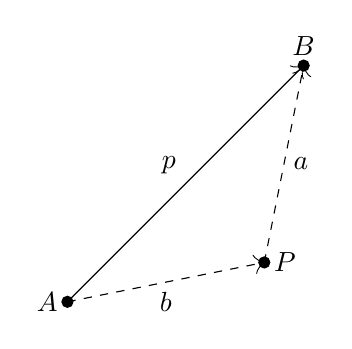
\begin{tikzpicture}
                \draw[dashed,-{Classical TikZ Rightarrow[scale=2]}] (-2,0) -- (0.5,0.5) node[midway, below] {$\vv b$};
                \draw[-{Classical TikZ Rightarrow[scale=2]}] (-2,0) -- (1,3) node[midway, above left] {$\vv p$};
                \draw[dashed,-{Classical TikZ Rightarrow[scale=2]}] (0.5,0.5) -- (1,3) node[midway, right] {$\vv a$};
                \draw[fill] (1,3) circle (2pt) node[above] {$B$};
                \draw[fill] (-2,0) circle (2pt) node[left] {$A$};
                \draw[fill] (.5,.5) circle (2pt) node[right] {$P$};
            \end{tikzpicture}
        \end{center}
        Define the vector from $A$ to $P$ as $\vv b$, from $A$ to $B$ as $\vv p$, from $P$ to $B$ as $\vv a$. Then, we need $\norm{\vv a} = \norm{\vv b}$.
        \begin{align*}
            \norm{\vv a} = \sqrt{(1+t-3)^2+(2-t-3)^2+(3+t-5)^2} &= 3 \\
            & t = 0 \qquad t = 2
        \end{align*}
        When $t=0$, $B=A$. Take $t=2$, then $B=(3,0,5)$
        
        \item We can find the middle point from the formula
        $$
        M = \left( \frac{1+3}{2}, \frac{2+0}{2}, \frac{3+5}{2} \right) = (2,1,4)
        $$
    \end{enumerate}
    
    \item Question 3
    \begin{enumerate}
        \item The planes are parallel. Plane 1 has a normal of $N_1=(1,-1,2)$, and Plane 2 has a normal of $N_2 = (2,-2,4)$. Take $k=2$, the we have $kN_1 = N_2$. This implies that $N_1$ is parallel to $N_2$. Since the normal of the two planes are parallel, the planes themselves are parallel as well.
        
        \item Let $A = (x,y,z) = (t,1+t,1-t)$ be the intersection point between the line and Plane 1. Then,
        \begin{align*}
            t-(1+t)+2(1-t) &= 5 \\
            t &= -2
        \end{align*}
        So $A=(-2,-1,3)$
        
        Similarly, let $B = (x,y,z) = (t,1+t,1-t)$ be the intersection point between the line and Plane 2. Then,
        \begin{align*}
            2t - 2(1+t) + 4(1-t) &= -10 \\
            t &= 3
        \end{align*}
        So $B=(3,4,-2)$.
        
        \item To find point $C$, we need to first find the line passing through $A$ that is perpendicular to Plane 2. We can define this line using $A$ and the normal of Plane 2.
        $$
        L:\, (-2,-1,3)+(2,-2,4)t
        $$
        Then find the intersection point between $L$ and Plane 2. Let $C=(-2+2t,-1-2t,3+4t)$. Since $C$ is on Plane 2,
        \begin{align*}
            2(-2+2t) - 2(-1-2t) + 4(3+4t) &= -10 \\
            t&=-20/24
        \end{align*}
        Substitute $t$ back to the coordinate of $C$ gives us $C=(-11/3,2/3,-1/3)$
    \end{enumerate}
    
    \item Question 4
    \begin{enumerate}
        \item 
        We want to show that $\norm{\vv u + \vv v}^2 + \norm{\vv u - \vv v}^2 = 2\norm{u}^2 - 2\norm{v}^2$.
    
        We begin from the left-hand side
        \begin{align*}
            \norm{\vv u + \vv v}^2 + \norm{\vv u - \vv v}^2 &= (\vv u + \vv v) \cdot (\vv u + \vv v) + (\vv u - \vv v) \cdot (\vv u - \vv v) \\
            & \text{by property of dot product} \\
            &= (\vv u \cdot \vv u + \vv u \cdot \vv v + \vv u \cdot \vv v + \vv v \cdot \vv v) + (\vv u \cdot \vv u - \vv u \cdot \vv v - \vv u \cdot \vv v + \vv v \cdot \vv v) \\
            & \text{by distributive property of dot product} \\
            &= \vv u \cdot \vv u + \vv u \cdot \vv u + \vv v \cdot \vv v + \vv v \cdot \vv v \\
            & \text{by associative property of dot product} \\
            &= 2\norm{\vv u}^2 + 2\norm{\vv v}^2 \\
            & \text{by property of dot product}
        \end{align*}
        Since $LHS=RHS$, this identity is holds.
        
        \item Assume that $\vv u$, $\vv v$ and $\vv u \times \vv v$ are all unit vectors. By property of cross product,
        $$
        \sin\theta = \frac{\norm{\vv u \times \vv v}}{\norm{\vv u}\norm{\vv v}}
        $$
        where $\theta$ is the angle between the two vectors.
        
        To find $\theta$ we use the inverse sine function:
        $$
        \theta = \sin^{-1}\left( \frac{\norm{\vv u \times \vv v}}{\norm{\vv u}\norm{\vv v}} \right)
        $$
        Since $\vv u$, $\vv v$ and $\vv u \times \vv v$ are all unit vectors, their norms are all 1. So $\theta = \sin^{-1}1/1 = 90\degree$
    \end{enumerate}
    \item Question 5
    \begin{enumerate}
        \item We first find the parametric equation for $L_1$.. 
        
        For $L_1$, we have the points $(1,0,1)$ and $(4,-2,2)$. The direction vector $\vv d_1 = (3,-2,1)$. Then, the equation for $L_1$ is $(1,0,1) + (3,-2,1)t$.
        
        Let $A$ be the intersection point between $L_1$ and $P_1$. Since $A$ is on $L_1$, $A=(1+3t,-2t,1+t)$. And since $A$ is on $P_1$,
        \begin{align*}
            (1+3t)+(-2t)+(1+t) &= 1 \\
            t &= -0.5
        \end{align*}
        Then, $A=(-0.5,1,0.5)$.
        
        Let $B$ be the intersection point between $L_1$ and $P_1$. Since $B$ is on $L_1$, $B=(1+3t,-2t,1+t)$. And since $B$ is on $P_1$,
        \begin{align*}
            (1+3t)+-2(-2t)+3(1+t) &= 5 \\
            t &= 0.1
        \end{align*}
        Then, $B=(1.3,-0.2,1.1)$.
        
        \item The angle between the planes $P_1$ and $P_2$ is the same as the angle between their normal, which can be found using dot product.
        $$
        \theta = \cos^{-1} \left( \frac{(1,1,1) \cdot (1,-2,3)}{\norm{(1,1,1)} \norm{(1,-2,3)}} \right) = 72.02\degree
        $$
        
        \item Let $\vv d = (x,y,z)$ be the direction vector of the line of intersection of $P_1$ and $P_2$. Then, $\vv d$ must be perpendicular to the normal of both planes, namely
        $$
        \vv d \cdot N_1 = 0 \quad \text{and} \quad \vv d \cdot N_2 = 0
        $$
        Substitute the values of $\vv d, N_1, N_2$.
        $$
        (x,y,z) \cdot (1,1,1) = 0 \qquad (x,y,z) \cdot (1,-2,3)
        $$
        Solving this gives $\vv d = (5,-2,-3)$.
        
        We also need another point $P_0$ that is on both planes. One of such point is $P_0 = (4,-2,-1)$. From $P_0$ and $\vv d$, we can define the line as
        $$
        L:\, (4,-2,-1) + (5,-2,-3)t
        $$
        which in symmetric form is
        $$
        \frac{x-4}{5} = \frac{y+2}{-2} = \frac{z+1}{-3}
        $$
    \end{enumerate}
    
    \item Question 6
    \begin{enumerate}
        \item To find the point on a plane that is closest to another point, we need to find the line passing through that external point that is also perpendicular to the plane. We can find such line using the coordinate of the external point and the normal of the plane.
        
        For $P_1$, define the line $L_1$ as
        $$
        L_1:\, (2,-3,4)+(1,-1,1)t
        $$
        where $(1,-1,1)$ is the normal of the plane.
        
        Then, we can find $P_1$ by solving for the intersection point of $L_1$ and the plane. Let $P_1$ be such intersection point, then since $P_1$ is on $L_1$, $P_1=(2+t,-3-t,4+t)$ for some scalar $t$. And since $P_1$ is also on the plane, it must satisfy that
        \begin{align*}
            (2+t) - (-3-t) + (4+t) &= -3 \\
            t &= -4
        \end{align*}
        Then, $P_1=(-2,1,0)$.
        
        Similarly, $L_2:\, (2,-3,-4)+(1,-1,1)t$ and $P_2=(2+t,-3-t,-4+t)$ for some scalar $t$. Since $P_2$ is also on the plane,
        \begin{align*}
            (2+t) - (-3-t) + (-4+t) &= -3 \\
            t &= -4/3
        \end{align*}
        Then, $P_2=(2/3, -5/3, -16/3)$.
        
        \item
        Define the following points
        $$
        A=(2,-3,4) \qquad B=(2,-3,-4) \qquad C=(-2,1,0) \qquad D=(2/3,-5/3,-16/3)
        $$
        vectors
        \begin{align*}
            \vv{AC} &= (-4,4,-4)\\
            \vv{AB} &= (0,0,-8)\\
            \vv{DC} &= (-2.67,2.67,5.33)\\
            \vv{DB} &= (1.33,-1.33,1.33)\\
        \end{align*}
        Divide the polygon into two triangles, areas of which can be found using cross products.
        \begin{align*}
            A_{ABDC} &= A_{ABC} + A_{CDB} \\
            &= \left\lVert \frac{\vv{AC} \times \vv{AB}}{2} \right\rVert + \left\lVert \frac{\vv{DC} \times \vv{DB}}{2} \right\rVert \\
            &= 30.17
        \end{align*}
    \end{enumerate}
    
    \item Question 7
    \begin{enumerate}
        \item To show the planes are parallel, it suffices to prove that their normals are parallel. The normal $N_1$ for $PL_1$ is $(2,-1,3)$. And the normal for $PL_2$ is $N_2 = (10,-5,15)$. Take $k=5$. Then, $kN_1=N_2$, which implies that $N_1$ is parallel to $N_2$. Since the normals are parallel, $PL_1$ is parallel to $PL_2$.
        
        \item Substitute the coordinate of $P$ into the equation of $PL_2$.
        $$
        10\cdot (-2) -5 \cdot 2 + 15 \cdot 2 = -20-10+30 = 0
        $$
        which is equal to the right-hand side of the equation of $PL_2$. Therefore, $P$ is on the plane $PL_2$.
        
        \item The equation of this sphere is
        $$
        (x+2)^2 + (y-2)^2 + (z-2)^2 = r^2
        $$
        We need to find the radius of the sphere. To do that, we find the distance between the point and the plane. This can be done using the formula
        $$
        r=D=\frac{|ax_1+by_1+cz_1+d|}{\sqrt{a^2+b^2+c^2}} = \frac{2\cdot (-2) + (-1)\cdot2 + 3\cdot2}{\sqrt{2^2 + (-1)^2 + 3^2}} = 2
        $$
        Then the equation of the sphere is
        $$
        (x+2)^2 + (y-2)^2 + (z-2)^2 = 4
        $$
    \end{enumerate}
    
    \item Question 8
    Let $A=(-3,3,-7)$, $B=(-1,2,-4)$, $C=(1,1-1)$, and $D=(5,-1,5)$. Define the following vectors
    $$
    \vv{AB} = (2,-1,3) \qquad \vv{BC}=(2,-1,3) \qquad \vv{CD}=(4,-2,6)
    $$
    \begin{enumerate}
        \item Using parallel vectors
        
        $$
        2\vv{AB}=\vv{CD} \qquad 1\vv{AB}=\vv{BC}
        $$
        Then $\vv{AB} \parallel \vv{CD}$ and $\vv{AB} \parallel \vv{BC}$. Since the parallel relation is transitive $\vv{AB}$ is parallel to $\vv{CD}$ which is also parallel to $\vv{BC}$. Since those vectors are parallel, $A,B,C,D$ are co-linear.
        
        \item Using triple product
        
        The triple product of the three vectors gives the volume of the parallelepiped defined by the three vectors. If the volume is zero, this implies that the points from which we defined the vectors are co-linear.
        
        Compute the triple produt
        $$
        \vv{AB} \cdot (\vv{AC} \times \vv{AD}) = 0
        $$
        Since the volume of the parallelepiped defined by the three vectors is zero, then the points must be co-linear.
        
        \item Using distance formula
        
        Calculate the following distances
        \begin{align*}
            AB &= \sqrt{2^2+(-1)^2+3^2} = \sqrt{14} \\
            BC &= \sqrt{2^2 + (-1)^2 + 3^2} = \sqrt{14} \\
            CD &= \sqrt{4^2+(-2)^2+6^2} = 2\sqrt{14} \\
            AD &= \sqrt{(5+3)^2 + (-1-3)^2 +(5+7)^2} = 4\sqrt{14}
        \end{align*}
        Since $AB+BC+CD=AD$, the points are co-linear.
        
        \item Using equation of a line.
        
        Define a line using points $A$ and $B$.
        $$
        L:\, (-1,2,-4)+(2,-1,3)t
        $$
        There exists $t=1$ such that $(-1,2,-4)+(2,-1,3)=(1,1,-1)=C$; and $t=3$ such that $(-1,2,-4)+3(2,-1,3)$. This implies that $C$ and $D$ are both on the line defined by $A$ and $B$. Therefore, the points are co-linear.
    \end{enumerate}
\end{enumerate}

\end{document}